\documentclass[a4paper,10pt,twoside]{article}

\setlength{\parskip}{2mm}


\usepackage[utf8]{inputenc}
\usepackage{amsfonts}
\usepackage{amsmath}
\usepackage{mathpazo}
\usepackage{multicol}
\usepackage{amssymb}
\usepackage{amsthm}
\usepackage{setspace}
\usepackage{fancybox}
\usepackage[spanish]{babel}
\usepackage[T1]{fontenc}
\usepackage[pdftex]{graphicx} %Utilizarlo sólo si voy a compilar con pdftex y tengo imágenes pixeladas (no vectoriales) con las gráficas.
\usepackage{cancel}
\usepackage{fancyhdr}
\usepackage{eurosym}
% \usepackage[dvips]{graphicx}%Utilizarlo para  cargar archivo de extensión *.eps (gráficos vectoriales)en el documento
\DeclareGraphicsExtensions{.png,.pdf,.jpg}
% \usepackage{pstricks-add}%Utilizarlo para cargar código ps-tricks de geogebra por ejemplo (no usar con
% \usepackage[pdftex]{graphicx})
\usepackage[colorlinks=true,linkcolor=blue]{hyperref}
\usepackage{hyperref}
\hypersetup{
    colorlinks,%
    citecolor=black,%
    filecolor=black,%
    linkcolor=black,%
    urlcolor=black
}
\usepackage{wrapfig}
\usepackage{textcomp}
\usepackage{nonfloat}%para poder poner notas al pie en los pies de Figuras o de Tablas
                     %\begin{minipage}{\textwidth}
                     %   \centering
                     %   \begin{tabular}{|c|}
                     %      \hline  Tabular stuff here \\ \hline
                     %   \end{tabular}
                     %   \tabcaption[Text of the caption (second example)]{Text of the caption (second example)\footnotemark}
                     % \end{minipage}
                     % \\[\intextsep]
                     %\footnotetext{Text of the footnote (second example)}
\usepackage{colortbl}%Para colores en tablas
\usepackage{verbatim} %Para utilizar comentarios comentarios

%Nueva geometría de la página, con respecto a la de por defecto
\usepackage[text={14.7cm,22.6cm},centering]{geometry}
\addtolength{\headsep}{-0.35cm}
\addtolength{\footskip}{-0.3cm}
\addtolength{\voffset}{0.6cm}%{-0.65cm}
\addtolength{\hoffset}{-0.05cm}%{-0.65cm}


%%%%% Para los encabezados y pies de Página
\pagestyle{fancy}
\lhead[\scriptsize{\textit{\href{mailto:asalber@ceu.es}{Alfredo Sánchez Alberca}}}]{\scriptsize{\textit{Innovación
en la docencia de Estadística con R y rk.Teaching}}}
% a completar por equipo editorial
\chead{}
\rhead[\scriptsize{\textit{Sección de la Revista}}]{\scriptsize{\textit{\href{mailto:mailautor@xxxx.es}{Nombre y Apellidos del Autor}}}} % a completar por equipo editorial
\lfoot[\thepage \ \  |  \ \scriptsize{\textit{Revista ``Pensamiento Matemático''}}]{\scriptsize{\textit{Volumen X, Número X, Xxx'XX, ISSN 2174-0410}}}% a completar por equipo editorial
\cfoot{}
\rfoot[\scriptsize{\textit{Volumen X, Número X, Xxx'XX, ISSN 2174-0410}}]{\scriptsize{\textit{Revista ``Pensamiento Matemático''}}\ \ \ \normalsize{|} \   \thepage}
%%%%% Fin de encabezados y pies de página

%%%%% Genera los pies de Figuras y Tablas en itálicas y a tamaño footnote
\usepackage[font={footnotesize,it}, format=plain, labelformat=simple, labelsep=period, center]{caption}
\renewcommand\thefigure{\arabic{figure}} % Genera numeración X
\renewcommand\thetable{\arabic{table}} % Genera numeración X

\setcounter{page}{1}%para comenzar la numeración de las páginas en documentos. Dejar 1 por defecto.

% Definición de comandos
\newcommand{\rkteaching}{\textsf{rk.Teaching}}
\newcommand{\rkward}{\textsf{RKWard}}
\newcommand{\spss}{\textsf{SPSS}}
\newcommand{\statgraphics}{\textsf{Statgraphics}}


\begin{document}
%Cambiar Palabra Cuadros por Tablas
\renewcommand{\tablename}{Tabla} 

\title{\vspace{-8mm}Sección de la Revista\\\vspace{4mm}
Innovación en la docencia de Estadística\\ con R y rk.Teaching\\\vspace{4mm}
Innovation in teaching Statistics\\ with R and rk.Teaching\vspace{-3mm}}  %Para poner el título del artículo
\author{\href{mailto:asalber@ceu.es}{Alfredo Sánchez Alberca}\\ \vspace{2mm} %pone el nombre del autor
\scriptsize Revista de Investigación\\
\small
\href{http://www2.caminos.upm.es/Departamentos/matematicas/revistapm/}{\includegraphics[width=75.2mm]{logosrev.png}}\\
\scriptsize Volumen X, Número X, pp. xxx--yyy, ISSN 2174-0410\vspace{-2mm}\\ 
\scriptsize Recepción: XX Xxx'XX; Aceptación: XX Xxx'XX} %xxx-yyy son las páginas inicial y final respectivamente
\date{23 de mayo de 2016}
%indispensable que al compilarlo se tenga en el mismo directorio raíz el archivo logomirinconbyn.eps que facilito en la descarga.
\maketitle

\begin{abstract}
En los últimos años el departamento de Matemática Aplicada y Estadística de la Universidad CEU San Pablo ha hecho una
apuesta decidida por el uso del software libre, y en particular de R, en la docencia de Estadística. 
Para ello se ha desarrollado el paquete \rkteaching{} con el objeto de superar las limitaciones de las interfaces
gráficas de usuario de R existentes hasta la fecha y liberar a los alumnos de la necesidad de aprender a programar R. 

En este artículo se presentan las principales características del paquete \rkteaching{} y se valora uso docente en las
clases prácticas de Estadística tanto presenciales como no presenciales.

\newline
\noindent\textbf{Palabras Clave:} Estadística, Análisis de Datos, Docencia, R, \rkteaching.
\newline
\begin{center}
 \textbf{Abstract}
\end{center}

\vspace{1.2mm}A translation of the abstract in english.\\
\newline
\noindent\textbf{Keywords:} Statistics, Data Analysis, Teaching, R, \rkteaching.

\end{abstract}

\section{Introducción}
\label{s:introduccion}
En las últimas décadas, el uso software estadístico para el análisis de datos se ha convertido en una práctica
generalizada en todas las titulaciones experimentales.
Hoy en día, prácticamente nadie concibe la aplicación de los procedimientos estadísticos y los cálculos que estos
requieren sin ayuda de un ordenador, sobre todo cuando el volumen de datos es ingente.
Es por ello que prácticamente todos los grados con alguna asignatura de Estadística incluyen talleres o clases prácticas
donde los alumnos aprenden a manejar algún programa de análisis de datos que les permite abstraerse de los tediosos
cálculos y centrarse en el análisis de los resultados.

La Universidad CEU San Pablo es una de las pioneras en introducción del software estadístico en sus titulaciones. 
Desde hace más de dos décadas se han utilizado diversos programas de análisis de datos como
Excel\footnote{\url{http://office.microsoft.com/es-es/excel/}},
\statgraphics{}\footnote{\url{http://www.statgraphics.net/}} o
\spss{}\footnote{\url{http://www-01.ibm.com/software/es/analytics/spss/}} para la docencia de la Estadística en
titulaciones de Ciencias de la Salud como Medicina, Farmacia, Psicología, Fisioterapia, Enfermería, Óptica y Nutrición.

Como es lógico, estos programas han ido mejorando a lo largo del tiempo y ofreciendo cada vez más posibilidades y
facilidades para el usuario, por lo que poco a poco han ido adquiriendo más protagonismo en las clases de Estadística.
Sin embargo, la mayoría de estos programas no han sido concebidos para la docencia, sino más bien para ser utilizados
por usuarios que ya tienen unos conocimientos mínimos de Estadística.

Por otro lado, casi todos ellos, o al menos lo más extendidos en el ámbito profesional, no son software libre.
Esto supone, en primer lugar, que los usuarios deben pagar una licencia para poder usarlos, algo que no todos los
alumnos pueden afrontar, sobre todo en el caso de \spss{} que tiene un precio prohibitivo para pequeños usuarios.
Y en segundo lugar, que no se puede acceder al código fuente, por lo que no pueden adaptarse a las necesidades docentes.

Por tal motivo, el departamento de Matemática Aplicada y Estadística de la Universidad CEU San Pablo se
planteó en 2008 el cambio al software libre en la docencia de Estadística.
Y así se empezó a utilizar R, que era el programa de análisis de datos libre más extendido en la comunidad
científica, en las clases prácticas de Estadística de las titulaciones de Farmacia y Medicina.

R\footnote{\url{http://www.r-project.org/}} \cite{r2001language} es una implementación de código abierto del
lenguaje de análisis de datos S.
Al tratarse de un lenguaje de programación especialmente pensado para el tratamiento y análisis de datos, es fácilmente
ampliable mediante nuevas funciones y procedimientos que suelen distribuirse en forma de paquetes de código abierto.
Esto lo hace sumamente potente ya que cuando el usuario requiere un procedimiento que no está implementado, siempre
puede programarlo él mismo y compartirlo con la comunidad para que otros también puedan beneficiarse de él.
R cuenta de hecho con una colección de paquetes de código abierto que están organizados en el repositorio Comprehensive
R Archive Network (CRAN), que, a fecha de escritura de este artículo, cuenta con 8447
paquetes\footnote{\url{http://cran.r-project.org/web/packages/}}.
Estos paquetes implementan los procedimientos estadísticos más habituales para el análisis de datos, pero también los
más avanzados y novedosos, superando con creces incluso a \spss{}, lo que ha hecho de R el software libre de análisis de
datos más extendido entre la comunidad científica.

Sin embargo, el principal inconveniente que presentaba R para su uso en la docencia era la falta de una interfaz
gráfica de usuario (GUI) que evitase a los alumnos tener que usar la línea de comandos y, en definitiva, aprender a
programar en R; algo sumamente útil, pero que tiene una de aprendizaje pronunciada. 

Así pues, el principal reto que nos marcamos fue el de conseguir una interfaz gráfica de usuario que le resultase a los
alumnos al menos tan fácil de manejar como la de los otros programas que habían utilizado hasta entonces.
Pero además lo suficiente versátil como para adaptarla a la visión que tenían los profesores del departamento de la
asignatura de Estadística y a las necesidades docentes en cada una de las titulaciones.

En el resto del artículo se cuenta cómo se afrontó este reto mediante el uso de la interfaz gráfica \rkward{} y el
desarrollo de un paquete de R específico para la docencia de Estadística, el paquete \rkteaching. 
En la sección~\ref{s:rkward} se presenta la interfaz gráfica de usuario \rkward{} y los motivos de su elección. 
En la sección~\ref{s:rkteaching} se describe el paquete \rkteaching{} y las características que lo hacen tan interesante
para la docencia de Estadística. 
En la sección\ref{s:docencia} se cuenta brevemente la experiencia docente del uso de rk.Teaching en las clases de
Estadística y la notable mejora tanto en el aprendizaje de los alumnos como en la eficiencia de uso del software por
parte de estos. 
Finalmente la sección~\ref{s:conclusiones} cierra el artículo con las principales conclusiones y posibles líneas de
investigación para seguir innovando.


\section{La interfaz gráfica de usuario \rkward}
\label{s:rkward}
Cuando se tomó la decisión de usar R en las clases de Estadística, las interfaces gráficas que existían por aquel
entonces eran aún muy primitivas y poco maduras.
Las principales características que requeríamos para una interfaz gráfica de usuario era que fuese amigable,
multiplataforma, configurable y ampliable para adaptarla a nuestras necesidades.

En un primer momento se optó por \textsf{R Commander} \cite{fox2005r}, que fue la primera interfaz gráfica orientada a
usuarios no expertos, multiplataforma y ampliable mediante un sistema de plugins.
\textsf{R Commander} se utilizó durante dos años en las clases de Estadística de las titulaciones de Farmacia y
Medicina.
Sin embargo, \textsf{R Commander} no estaba a la altura de las interfaces gráficas mucho más maduras de \statgraphics{} o
\spss{}, por lo que a los alumnos les costó aceptar el cambio. 

Mientras tanto, en 2002 Thomas Friedrichsmeier había comenzado el desarrollado de
\rkward{}\footnote{\url{http://rkward.sourceforge.net/}} \cite{rodiger2012rkward}, otra interfaz gráfica de usuario de
código abierto basado en las librerías KDE y Qt, mucho más modernas y con un aspecto visual más homogéneo.
Pero \rkward{} no era multiplataforma y sólo estaba disponible para sistemas Linux en un principio.
No obstante, en 2010 se anuncia por fin la versión 0.5.5 de \rkward{} que ya era multiplataforma (disponible para
Windows, Mac y Linux) y rápidamente se opta por empezar a usarla en lugar de \textsf{R Commander}.
Poco después surgirá la interfaz \textsf{RStudio}\footnote{\url{https://www.rstudio.com/}}, que en estos últimos
años se ha extendido con mucha más fuerza que \rkward{} convirtiéndose en la interfaz gráfica de usuario para R más
utilizada incluso en el ámbito universitario.
Sin embargo, la principal ventaja de \rkward{} frente a \textsf{RStudio}, y que hizo que nos decantásemos por esta
primera, es que es fácilmente ampliable mediante un sistema de plugins (complementos) que permiten añadir menús y
cuadros de diálogo con nuevos procedimientos estadísticos \cite{friedrichsmeier2011introduction}, algo fundamental para
nuestros propósitos ya que nos otorgaba la versatilidad que buscábamos para poder adaptar la herramienta a nuestras
necesidades docentes.

Pero además de esto, \rkward{} disponen de otras muchas características que lo hacen muy interesante, entre las que cabe
destacar que dispone de menús y cuadros de diálogos para realizar los análisis de datos más habituales sin necesidad de
conocer el lenguaje R, tal y como se aprecia en la figura~\ref{f:ventana-datos-rkward}; pero al mismo tiempo es un
completo entorno de desarrollo en R para programadores experimentados con su propia consola de ejecución y depuración.
Además el usuario puede ver si lo desea el código R asociado a los menús y las opciones seleccionadas en los
cuadros de diálogos de los distintos procedimientos estadísticos, tal y como se muestra en la
figura~\ref{f:codigo-test-t}, algo que resulta muy valioso para los usuarios que quieren aprender el lenguaje R.

\begin{figure}[htbp!]
\centering
\includegraphics[width=\textwidth]{img/ventana_datos_rkward.png}
\caption{Ventana de entrada de datos de la interfaz gráfica de usuario \rkward{}.}
\label{f:ventana-datos-rkward}
\end{figure}

\begin{figure}[htbp!]
\centering
\includegraphics[width=\textwidth]{img/codigo_t_test.png}
\caption{Código R generado por \rkward{} para el procedimiento del test T de comparación de medias de poblaciones
independientes.}
\label{f:codigo-test-t}
\end{figure}

Finalmente, la salida que ofrece \rkward{} es en formato html, lo cual permite aplicar un formato mucho más rico a los
resultados de los análisis, así como insertar gráficos de forma sencilla y poder visualizarlo en cualquier navegador web.
 

\section{El paquete \rkteaching}
\label{s:rkteaching}
Aunque \rkward{} incorpora en sus menús los procedimientos estadísticos más comunes para el análisis de datos, estos
están pensados para usuarios expertos o al menos conocedores de los procedimientos y de los parámetros requeridos por
cada uno de ellos. 
Esto hace que los cuadros de diálogo correspondientes a cada procedimiento sean demasiado farragosos y poco intuitivos
para alumnos que están aprendiendo el uso de estos procedimientos.
Al mismo tiempo las salidas de los procedimientos son bastante sintéticas y difíciles de interpretar para usuarios
noveles. 

Por tal motivo, aprovechando la modularidad de \rkward, se decidió crear un plugin específico para la docencia de
Estadística que se adaptase más al perfil de usuario principiante de los alumnos universitarios que están aprendiendo
Estadística y que facilitase su aprendizaje. 
Con esta idea surgió el paquete de R \rkteaching\footnote{\url{http://aprendeconalf.es/rkteaching}}.
El objetivo que nos marcamos no sólo era desarrollar una interfaz gráfica de usuario amigable, que permitiera a los
alumnos utilizar R para realizar sus análisis de forma similar a como lo hacían hasta entonces con \spss{} o \statgraphics{},
sino hacer su uso incluso más intuitivo y desarrollar nuevos procedimientos que no estaban soportados por estos
programas. 

Así, los principios de diseño que han guiado el desarrollo de \rkteaching{} son la intuición, la simplicidad, la
asistencia al usuario, la interpretación de resultados y la pedagogía.  
Para ilustrar estos principios tomemos, por ejemplo, el procedimiento estadístico del test T para la comparación de
medias de dos poblaciones independientes.

\begin{description}
\item[Intuición] En primer lugar, los menús de \rkteaching{} están estructurados en bloques lógicos que facilitan la
localización de los distintos procedimientos estadísticos casi sin necesidad de ayuda, tal y como se muestra en la
figura~\ref{f:menu-test-t}.

\begin{figure}[htbp!]
\centering
\includegraphics[width=0.7\textwidth]{img/menu_test_t.png}
\caption{Estructura de menús de \rkteaching.}
\label{f:menu-test-t}
\end{figure}

Del mismo modo los cuadros de diálogo de cada menú tienen una estructura lógica y homogénea que dirige al usuario hacia
los campos que debe rellenar para cada procedimiento estadístico. 
Los campos más importantes a rellenar aparecen siempre en primer lugar y resaltados, mientras que los campos secundarios
u opcionales están ocultos o no admiten la entrada de valores hasta que se activan explícitamente. 
Además, los campos de entrada de variables están configurados para impedir que se introduzcan variables de tipos no
apropiados. 

\item[Simplicidad] Por otro lado, los cuadros de diálogo han sido diseñados para ser lo más simple posibles,
eliminando las opciones más complejas que se han considerado prescindibles en los procedimientos estadísticos
habituales, tal y como se muestra en la figura~\ref{f:dialogo-test-t}.

\begin{figure}[htbp!]
\centering
\includegraphics[width=0.8\textwidth]{img/dialogo_test_t.png}
\caption{Cuadro de diálogo de \rkteaching{} para el test T de comparación de medias de poblaciones independientes.}
\label{f:dialogo-test-t}
\end{figure}

Este es una de las mayores dificultades detectadas en otros programas como \spss{} en el que los
cuadros de diálogo de algunos procedimientos incorporan tal multitud de opciones que acaban por desorientar a los
alumnos alejándolos de lo esencial.


\item[Asistencia al usuario] Una de las principales ventajas de \rkteaching{} es el asistente de usuario. 
Todos los cuadros de diálogo incorporan un asistente que dirige al usuario paso a paso a través de las
distintas opciones que debe seleccionar para realizar cada procedimiento estadístico, tal y como se puede apreciar en la
figura~\ref{f:asistente-test-t}.

\begin{figure}[htbp!]
\centering
\includegraphics[width=\textwidth]{img/asistente_test_t.png}
\caption{Asistente de \rkteaching{} para el test T de comparación de medias de poblaciones independientes.}
\label{f:asistente-test-t}
\end{figure}

De este modo, si el usuario duda ante la información requerida por un cuadro de diálogo, puede solicitar
ayuda al asistente, que no sólo le informará del propósito del procedimiento estadístico seleccionado, sino que le
guiará en cada una de las decisiones requeridas en el procedimiento.

\item[Interpretación de resultados] Por último, pero no menos importante, las salidas tanto textuales como gráficas
de los procedimientos estadísticos que ofrece \rkteaching{} han sido cuidadosamente diseñadas para facilitar al máximo
la interpretación de los resultados. 
Esta es, probablemente, la parte más crítica y que más dificultad supone para los alumnos, que muchas veces son
capaces de seguir los pasos necesarios para realizar el procedimiento estadístico, pero luego no son capaces de
interpretar adecuadamente los resultados y sacar conclusiones apropiadas. 
Así, para facilitar la interpretación de los resultados las salidas se han estructurado de manera que al
comienzo siempre se muestra un resumen del procedimiento con las principales opciones seleccionadas, y
después se presentan los resultados en un orden lógico, mostrando exclusivamente la información relevante
a la hora de interpretar o tomar decisiones, tal y como se observa en la figura~\ref{f:salida-test-t}. 

\begin{figure}[htbp!]
\centering
\includegraphics[width=\textwidth]{img/salida_test_t.png}
\caption{Salida de \rkteaching{} para el test T de comparación de medias de poblaciones independientes.}
\label{f:salida-test-t}
\end{figure}

Además, al final de la salida se incluye una interpretación detallada del los resultados del procedimiento y las
principales conclusiones del mismo.
Por último, también se incluye un enlace al manual de estadística\footnote{\url{http://aprendeconalf.es/statistics/manual/}} utilizado en
clase por si el alumno necesita más información sobre el procedimiento estadístico aplicado. 

\item[Pedagogía] Finalmente, el principal principio que ha dirigido el diseño de \rkteaching{} ha sido el facilitar al
alumno el aprendizaje de la Estadística.
Así, además de hacer los menús y cuadros de diálogo simples e intuitivos, de ofrecerle ayuda mediante un asistente y de
facilitarle la interpretación de los resultados, \rkteaching{} incorpora para algunos procedimientos estadísticos el
detalle de los cálculos y las fórmulas usadas para facilitar su comprensión.
En la figura~\ref{f:calculo-detallado} se puede observar el cálculo detallado de la media y la varianza.
Esto permite, entre otras cosas, que un alumno que está realizando los cálculos a mano, pueda comprobar si lo está
haciendo bien o no.

\begin{figure}[htp]
\begin{center}
\includegraphics[width=\textwidth]{img/calculo_detallado.png}
\caption{Salida de \rkteaching{} con el cálculo detallado de la media y la varianza.}
\label{f:calculo-detallado}
\end{center}
\end{figure}

Por otro lado, algunos procedimientos gráficos son interactivos, lo que permite que el alumno interactúe con el cuadro
de diálogo cambiando algunas opciones al tiempo que ve los cambios que producen en la salida gráfica.
De este modo, el alumno puede comprender más fácilmente el papel de la media y la desviación típica en la distribución
normal al ver cómo cambia la forma de la campana de Gauss en una distribución normal al variar la media o la desviación
típica; comprobar para qué valores de $n$ y $p$ se puede aproximar una distribución binomial $B(n,p)$ mediante una
distribución Poisson $P(np)$ aplicando la Ley de los casos raros, tal y como se muestra en la
figura~\ref{f:ley-casos-raros}.

\begin{figure}[htp]
\begin{center}
\includegraphics[width=\textwidth]{img/ley_casos_raros.png}
\caption{Salida interactiva de \rkteaching{} para la Ley de los casos raros.}
\label{f:ley-casos-raros}
\end{center}
\end{figure}

Por último, \rkteaching{} también incorpora simulaciones que resultan esenciales para comprender determinados sucesos
probabilísticos como por ejemplo experimentos aleatorios con juegos de azar o el famoso teorema central del límite.  
\end{description}

Actualmente el paquete \rkteaching{} se encuentra en su versión 2.0 e incorpora los procedimientos descriptivos e
inferenciales más habituales en Estadística, desde la construcción de tablas y diagramas de distribución
de frecuencias, hasta los test paramétricos y no paramétricos más comunes. 
Incluye además procedimientos para el cálculo de probabilidades que no suelen incluirse en el software comercial, y
otros más específicos de Bioestadística como son los test diagnósticos. 
Por motivos de espacio no se incluye la lista completa de procedimientos incluidos en el paquete pero el lector
interesado puede obtenerla en \cite{asalber2016bringing} o en la propia página web del paquete
\url{http://aprendeconalf.es/rkteaching}.

Otra de las novedades de la última versión es que está disponible tanto en Castellano como en Inglés. 

\section{Experiencia docente con \rkteaching}
\label{s:docencia}
Desde su desarrollo, el paquete \rkteaching{} se ha utilizado en multitud de cursos tanto en docencia presencial como no
presencial. 

\subsection{Docencia presencial}
Durante los últimos seis años \rkteaching{} se usado para impartir las prácticas de Bioestadística en las titulaciones
de grado en Farmacia y Medicina de la Universidad CEU San Pablo.
Estas prácticas cubren todos los contenidos de la materia sin excepción (tabulación y representación gráfica de
distribuciones muestrales, cálculo de estadísticos descriptivos, regresión lineal y no lineal, cálculo de probabilidades
y test diagnósticos, distribuciones discretas y continuas de probabilidad, estimación de parámetros poblacionales
mediante intervalos de confianza, contrastes de hipótesis paramétricos y no paramétricos), algo que no ocurría con el
software anterior ya que ni \spss{}, ni \statgraphics{}, daban soporte a los contenidos de probabilidad.

Para facilitar la realización de las prácticas se ha elaborado el libro electrónico \emph{Bioestadística Aplicada
con R y rk.Teaching} \cite{sanchez2014bioestadistica}, que también se distribuye bajo una licencia libre. 
Este libro cubre todos contenidos antes mencionados con multitud de ejemplos prácticos aplicados a las Ciencias
Biosanitarias desarrollados paso a paso.

En estos años, la valoración de las prácticas de Estadística ha aumentado considerablemente por parte de los alumnos,
quienes agradecieron explícitamente el cambio experimentado con respecto a \textsf{R Commander}. 
De hecho, a tras los dos primeros años de uso se hizo un experimento para comparar la facilidad de uso y la satisfacción
de los alumnos con el nuevo software en comparación con \spss{}.
Los resultados concluyeron una eficiencia de \rkteaching{} al menos un 17\% superior a \spss{} y una falicidad de uso al
menos un 10\% superior \cite{sanchez2011rkteaching}.

La valoración de los docentes es si cabe más positiva aún ya que, gracias a la mayor eficiencia de \rkteaching{}, los
alumnos van más rápidos en la realización de las prácticas y asimilan mejor los contenidos. 
Esto ha permitido añadir una práctica más de probabilidad a los contenidos del curso, y aún así realizar las prácticas
más olgadamente que con el software anterior.

Otra de las mejoras significativas en la docencia tiene que ver con la evaluación de las prácticas.
Al finalizar las prácticas los alumnos tienen que hacer una trabajo práctico final aplicado a un caso real.
Antes de empezar a usar R y \rkteaching{} la corrección de este trabajo requería bastante tiempo a los profesores y
habitualmente se detectaban bastantes casos de plagio.
Ahora, sin embargo, la infraestructura que aporta R y \rkteaching{} nos ha permitido automatizar casi por completo tanto
la preparación como la corrección de este trabajo. 
Para cada curso se desarrolla un complemento que se integra en \rkteaching{} que permite a los alumnos generar unos
datos personalizados en función de su DNI, y una hoja de cálculo con un formulario en el que deben introducir las respuestas a
las preguntas planteadas.
Al finalizar el trabajo los alumnos suben la hoja de cálculo al campus virtual desde donde el profesor puede
descargarla y corregirla automáticamente de nuevo haciendo uso de un programa corrector implementado también en R.
Las notas y las hojas de cálculo corregidas se suben automáticamente de nuevo al campus virtual donde los alumnos pueden
consultarlas, y todo en un tiempo récord. 

\subsection{Docencia no presencial}
El paquete también se ha utilizado en varios cursos masivos abiertos en línea (MOOCs) de Bioestadística impartidos
en la plataforma Miríada X \cite{sanchez2013curso}.

\begin{figure}[htp]
\begin{center}
\href{https://youtu.be/BTFOsbzInZo}{\includegraphics[width=0.8\textwidth]{img/mooc.png}}
\caption{Vídeo promocional del curso MOOC de Bioestadística aplicada con R y rk.Teaching.}
\label{f:mooc}
\end{center}
\end{figure}

Hasta la fecha más de 5000 alumnos de todo el mundo se han inscrito en estos cursos y más de un 20\% han conseguido
terminarlos (un porcentaje por encima de la media en este tipo de cursos).
Estos cursos han sido unos de los mejores valorados en la plataforma Miriada X y se han recibido multitud de notas de
agradecimiento por parte de los inscritos que además pedían que se ampliase el curso con más contenidos. 
De momento los cursos sólo cubren la Estadística Descriptiva y la Regresión, pero ya se está preparando otro curso más
ambicioso de introducción a la investigación que cubre también la Estadística Inferencial. 

En los dos últimos años, el paquete \rkteaching{} también ha empezado a utilizarse, tanto presencial como no
presencialmente, en otras universidades entre las que se encuentra la Universidad Complutense, la Universidad Carlos III y la Universidad Rey Juan Carlos de Madrid.
En casi todos los casos se han interesado por el paquete como sustituto a \spss{} en las prácticas de Estadística de
distintas asignaturas.

Pero el interés por \rkteaching{} no sólo se limita al ámbito educativo, sino que hay multitud de usuarios e incluso
empresas que tras conocer el software a través del MOOC han empezado a usarlo a nivel profesional. 


\section{Conclusiones y futuras líneas de investigación}
\label{s:conclusiones}
El departamento de Matemática Aplicada y Estadística de la Universidad CEU San Pablo ha sido uno de los pioneros en
introducir el software de análisis de datos en la docencia de Estadística. 
En los últimos años el departamento ha hecho una apuesta decidida por el software libre, y en particular por R, en las
clases prácticas de Estadística. 
Para facilitar el uso de R a los alumnos, se ha desarrollado el paquete \rkteaching{} que, sobre la base de la interfaz
gráfica \rkward{}, proporciona menús y cuadros de diálogo amigables, sencillos e intuitivos para realizar los
procedimientos estadísticos requeridos en los cursos de Estadística impartidos. 

El paquete \rkteaching{} se ha utilizado durante los últimos seis años en las clases prácticas de Estadística de las
titulaciones de Farmacia y Medicina y también en varios cursos masivos en línea, con gran aceptación por parte de los
alumnos y una valoración muy favorable de los docentes.
Con esto se elimina la principal reticencia existente hasta ahora al uso de R en la docencia, que no era otra que la
falta de una interfaz gráfica de usuario similar a las ofrecidas por el software propietario, y que no obligase a tener
que programar en R.
\rkward{} en combinación con \rkteaching{} se puede considerar ya una interfaz gráfica de usuario de R lo
suficientemente madura para su uso en el ámbito de la docencia e incluso fuera de ella, llegando a superar incluso al
software propietario, y en particular \spss{}, tanto en eficiencia como en facilidad de uso como ha quedado
demostrado en varios experimentos realizados con los alumnos. 

El desarrollo del paquete \rkteaching sigue activo y actualmente se está trabajando en la mejora de las interpretaciones
de los resultados de los análisis y en incorporar procedimientos estadísticos más avanzados como algunas técnicas de
análisis multivariante. 
También se está desarrollando un nuevo curso MOOC de Estadística Inferencial para la introducción a la investigación
biosanitaria. 

\begin{thebibliography}{9}

\bibitem{friedrichsmeier2011introduction}
\textsc{Friedrichsmeier}, T., \textsc{Michalke}, M., \textit{Introduction to Writting Plugins
for RKWard}, 2011, \url{http://rkward.sourceforge.net/documents/devel/
-plugins/index.html} (accedido el 23 de mayo de 2016).

\bibitem{fox2005r}
\textsc{Fox}, J., \textit{The R Commander: A Basic-Statistsics Graphical User Interface to R}, Journal
of Statistical Software, Nº 14(9), 1--42.

\bibitem{r2001language}
\textsc{R Development Core Team}, \textit{R: A Language and Environment for Statistical Computing}, Viena: R Foundation
for Statistical Computing, 2001. 

\bibitem{rodiger2012rkward}
\textsc{Rödiger}, S., \textsc{Friedrichsmeier}, T., \textsc{Kapat}, P., \textsc{Michalke}, M., \textit{RKWard: A
Comprehensive Graphical User Interface and Integrated Development}, Environment for Statistical Analysis
with R. Journal of Statistical Software, Nº 49(9), pp. 1--34., 2012.

\bibitem{sanchez2011rkteaching}
\textsc{Sánchez-Alberca}, A., \textit{RKTeaching: Un paquete de R para la enseñanza de la Estadística}, Docencia en
Estadística. Experiencias de innovación (JIDERE), Nº 1, pp. 167--179, 2011.

\bibitem{sanchez2013rkteaching}
\textsc{Sánchez-Alberca}, A., \textit{RKTeaching: a new R package for teaching Statistics}, UseR!, Albacete, 2013. 

\bibitem{sanchez2013curso}
\textsc{Sánchez-Alberca}, A., \textit{Curso Práctico de Bioestadística con R}, Plataforma Miríada X.
\url{https://www.miriadax.net/web/ curso-practico-bioestadistica-r-3edicion} (accedido el 23 de mayo de 2016).

\bibitem{sanchez2014bioestadistica}
\textsc{Sánchez-Alberca}, A., \textit{Bioestadística Aplicada con R y RKTeaching}.
\url{http://aprendeconalf.es/estadistica/bioestadistica-rkteaching} (accedido el 23 de mayo de 2016).

\bibitem{sanchez2015bringing}
\textsc{Sánchez-Alberca}, A., \textit{Bringing R to non-expert users with the package RKTeaching}, Boletín de
Estadística e Investigación Operativa (BEIO), Nº 31-2, pp. 170--188, 2015.

\end{thebibliography}


\vspace{1cm}
\noindent\textbf{Sobre el autor:}\\
\emph{Nombre:} Alfredo Sánchez Alberca\\
\emph{Correo electrónico:} \href{mailto:asalber@ceu.es}{asalber@ceu.es}\\
\emph{Web:} \url{http://aprendeconalf.es}\\
\emph{Institución:} Universidad CEU San Pablo.\\
\emph{Departamento:} Matemática Aplicada y Estadística.

\end{document}